\documentclass[11pt]{article}
\usepackage{mathpazo}
\usepackage{url}
\usepackage[pdftex]{graphicx}
\usepackage{verbatim}

\newcommand{\vn}{\textsc{VN}}
\newcommand{\jf}{\textsc{jflap}}
\newcommand{\dt}{\textsc{dot}}
\newcommand{\spn}{\textsc{Spin}}
\newcommand{\prm}{\textsc{Promela}}
\newcommand{\erg}{\textsc{Erigone}}
\newcommand{\p}[1]{\texttt{#1}}
\newcommand{\bu}[1]{\textsf{#1}}

\textwidth=15cm
\textheight=20cm
\topmargin=0pt
\headheight=0pt
\oddsidemargin=1cm
\headsep=0pt
\renewcommand{\baselinestretch}{1.1}
\setlength{\parskip}{0.20\baselineskip plus 1pt minus 1pt}
\parindent=0pt

\title{\vn{} - Visualization of Nondeterminism\\User's Guide\\\mbox{}\\\large{Version 3.0}}
\author{Mordechai (Moti) Ben-Ari\\
Department of Science Teaching\\
Weizmann Institute of Science\\
Rehovot 76100 Israel\\
\textsf{http://stwww.weizmann.ac.il/g-cs/benari/}}
%\date{}
\begin{document}

\maketitle
\thispagestyle{empty}

\vfil

\begin{center}
Copyright (c) 2006-9 by Mordechai (Moti) Ben-Ari.
\end{center}
Permission is granted to copy, distribute and/or modify this document
under the terms of the GNU Free Documentation License, Version 1.2
or any later version published by the Free Software Foundation;
with Invariant Section ``Introduction,'' no Front-Cover Texts, and no Back-Cover Texts.
A copy of the license is included in the file \p{fdl.txt}
included in this archive.

\newpage

\section{Introduction}

\vn{} is a tool for studying the behavior of nondeterministic finite automata 
(NDFA). It takes a description of an automaton and generates a nondeterministic 
program; the program can then be executed randomly or guided interactively. The 
automaton and the execution path are graphically displayed.

\vn{} is written in Java for portability. It is based on other software tools: 
\begin{itemize}
\item The interactive editor of \jf{} is used to 
create an automaton, which is saved as an XML file that is the input to \vn{}. See: 
S. H. Rodger and T. W. Finley. \textit{JFLAP: An Interactive Formal 
Languages and Automata Package}. Jones \& Bartlett, 2006. \url{http://jflap.org/}.
\item The program generated from the automaton is written in 
\prm{}, the language of the \spn{} model checker. See: M. Ben-Ari. 
\textit{Principles of the Spin Model Checker}. Springer, 2008.
The program is run using the \erg{} model checker, which also uses
the \prm{} language. \url{http://code.google.com/p/erigone/}.
\item The graphical description of the automaton and path are created in the \dt{} 
language and layed out by the \dt{} tool. Graphs in PNG format are created and
are then displayed within \vn{}. \dt{} is part of the \textsc{Graphviz} 
package. \url{http://graphviz.org/}.
\end{itemize}

The \vn{} software is copyrighted according the the GNU General Public License.
See the files \p{copyright.txt} and \p{gpl.txt} in the archive.

The \vn{} webpage is \url{http://code.google.com/p/v-n/}.

\textbf{Acknowledgement:} Michal Armoni assisted in the design of \vn{}.

\section{Installation and execution}

\begin{itemize}
\item Install the Java SDK or JRE (\url{http://java.sun.com}).
\textbf{\vn{} needs Java 1.5 at least.}

\item For Windows: download the \vn{} installation file called \p{vn-N.exe},
where \p{N} is the version number, and execute the installation file.
For other systems, you will have to build \vn{}, and download and install
\erg{}, \dt{} and \jf{}.

\item The installation will create the following subdirectories: \p{docs} for the
documentation; \p{vn} for the source files; \p{bin} for the libraries and executables
for \erg{}, \dt{} and \jf{}; \p{txts} for the text files
(help, about and copyright); and \p{examples} for example programs.

\item To run \vn{}, execute the command \p{javaw -jar vn.jar}.
An optional argument names the \p{jff} file from \jf{} to be opened initially.
A batch file \p{run.bat} is supplied which contains this command.

\item Configuration data for \vn{} is given in the source file \p{Config.java}, 
as well as in the file \p{config.cfg}. The latter is reset to its default values
if it is erased.

\item To rebuild \vn{}, execute \p{build.bat}, which will compile all the source
files and create the file \p{vn.jar} with the manifest file.
\end{itemize}

\section{Interacting with \vn{}}

The display of the \vn{} program is divided into three scrollable panes. 
Messages from \vn{} are displayed in the text area at the bottom of the screen.
Graphs of automata are displayed in the left-hand pane and graphs of the paths 
are displayed in the right-hand pane. The size of the panes is adjustable and 
the small triangles on the dividers can be used to maximize a pane.
Above the panes is another text area called the path area
where execution paths of the automaton are displayed.

Interaction with VN is through a toolbar. All toolbar buttons have mnemonics 
(Alt-character).

\begin{figure}[htbp]
\begin{center}
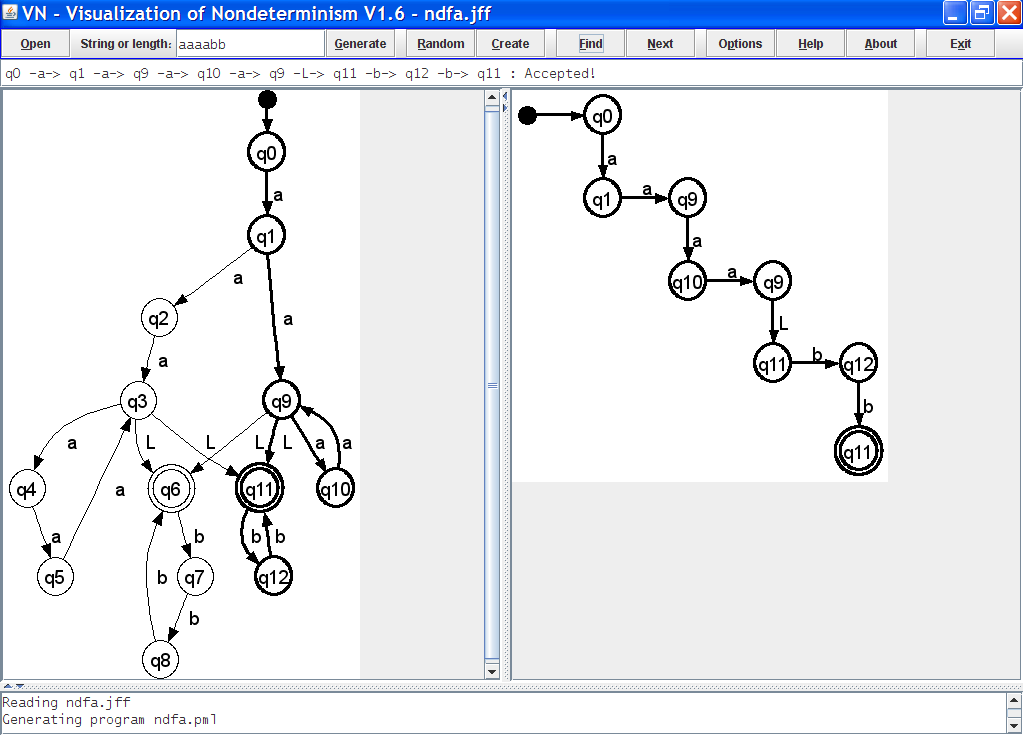
\includegraphics[width=.8\textwidth,keepaspectratio=true]{vn.png}
\end{center}
\end{figure}
 
\begin{description}
\item[\bu{Open}] Brings up a file selector; select a \p{jff} file and the 
automaton described in the file will be displayed.
\item[\bu{Edit}] This invokes \jf{} on the current automaton.
\textbf{The modified \p{jff} file must be re-opened in \vn{} after it is
saved in \jf{}.}
\item[\bu{String or length}] Enter an input string for the automaton in this text field.
See below on entering a length.
\item[\bu{Generate}] Once an automaton has be opened and an input string entered in 
the text field, selecting \bu{Generate} will create a program to execute the 
automaton.
\item[\bu{Random}] This will execute the program for the automaton with a 
random resolution of nondeterminism. The sequence of states will appear in the 
text area below the toolbar, along with an indication if the input string was 
accepted or rejected.
\item[\bu{Create}] This will execute the program for the automaton, resolving 
nondeterminism interactively. Determinisitic choices will be made 
automatically; if a choice cannot be taken, it will be displayed in square 
brackets and cannot be selected. \bu{Quit} terminates the execution. Keyboard 
shortcuts: \bu{Tab} moves between buttons and \bu{Space} or \bu{Enter} selects the 
highlighted button.
\item[\bu{Find}] This searches for an accepting computation of the automaton.
\item[\bu{Next}] This searches for the next accepting computation of the automaton.
When no more accepting computations exist, the number of accepting computations
is displayed in the path area.
\item[\bu{DFA}] See below.
\item[\bu{Options}] Displays a diaglog for choosing the size of the graphs
(small, medium, large) and whether the highlighting of the paths will be in
color or bold. When you select \bu{OK} the changes will be saved, 
along with the directory of the current open file.
\item[\bu{Help}] Displays a short help file.
\item[\bu{About}] Displays copyright information about the software. The 
version number appears in the title bar.
\item[\bu{Exit}] Exit the application.
\end{description}
Once a computation has been found , the path itself is displayed
in the right-hand pane and highlighted
in the automaton in the left-hand pane. The difference is that the 
``path'' includes multiple visits to the same state, while the highlighted path 
will, of course, include just one state for all occurences.

\noindent\textbf{Searching for all inputs that are accepted}

If you an integer value in the text field \bu{String or length},
each selection of \bu{Next}
searches for an accepting computation for \emph{any} input string of
this length. When no more accepting computations are found,
the set of strings that are accepted is displayed in path area.
For the automaton \p{ndfa.jff} supplied in the archive and with input length six, 
there are seven accepting computations for the four inputs:
\p{aaaaaa, aaaabb, aaabbb, aabbbb}.

\bigskip
\bigskip

\noindent\textbf{Equivalence classes of deterministic finite automata}

If the automaton is  deterministic, it is possible to obtain
the partition of a set of input strings of a given length
into the equivalence classes 
associated with each state.\footnote{This functionality was inspired by \bu{ProofChecker}:\\ \hspace*{2cm}\url{http://research.csc.ncsu.edu/accessibility/ProofChecker/index.html}.}
Enter a length in the text field and select \bu{Generate}.
Now select \bu{DFA} repeatedly;
for each state, starting from the first state, the set of input strings ``accepted'' by that
state is displayed. When \bu{DFA} has been selected for all states,
the set of equivalence classes is displayed in the right-hand pane.\footnote{\bu{Generate} 
can be selected at any time to reset to the first state.}

For the DFA in the \p{examples} directory, the equivalence classes
of length~$4$ are:
\begin{verbatim}
q0: [bbaa, baba, abba, aaaa]
q1: [bbab, babb, abbb, aaab]
q2: [bbba, baaa, abaa, aaba]
q3: [bbbb, baab, abab, aabb]
\end{verbatim}

\section{Files}
The different phases of processing \vn{} communicate through files. Here is a
list of the extensions of these files:
\begin{itemize}
  \item[\p{jff}] JFLAP XML description of an automaton
  \item[\p{pml}] Promela source generated from the automaton
  \item[\p{pth}] Path resulting from running \spn{} on the \p{pml} file
  \item[\p{dot}] Graphics file describing automaton and path
  \item[\p{png}] \textsc{PNG} graphics file after layout by \dt{}
\end{itemize}

\section{Software structure}
\p{VN} is the main class and contains declarations
of the GUI components and the event handler for all the buttons.

\p{Config} contains constants and properties.

\p{Options} displays a dialog for changing the size and highlight of the graphs.

\p{DisplayFile} displays the files for \bu{About} and \bu{Help}
in a \p{JFrame}.

\p{JFFFileFilter} is used with a \p{JFileChooser} to open a \p{jff} file.

\p{ImagePanel} displays the \textsc{PNG} files.

\p{GenerateSpin} generates the \prm{} program from the automaton.

\p{ReadXML} reads the XML description of the automaton from the \p{jff} file and
stores the data in \p{states} and \p{transitions}. These types are defined in
classes \p{State} and \p{Transition}.

\p{ReadPath} reads the path data printed by the \prm{} program and stores it in
\p{pathStates} and \p{pathTransitions}.

\p{WriteGraph} writes the automaton and paths in \dt{} format and forks a process to
run \dt{} to layout the graph.

\p{RunSpin} forks a process to execute \spn{}. In interactive mode, it reads the
\prm{} program so that the \p{JOptionPane} used for selecting among
nondeterministic choices can display actual source code. For \bu{Find} and
\bu{Next} processes are forked to run the C compiler and \p{pan}. 
For \bu{Next}, \p{pan} is run with the \p{-c} argument.

\appendix

\section{Release notes}

\begin{description}
\item[3.0] \erg{} is used as the model checker instead of \spn{}.
The previous versions will not be maintained.
\end{description}

\end{document}
